\documentclass[10pt,compress,serif]{beamer}
\usepackage{pres2023_169}
\usepackage[utf8]{inputenc}
 
\renewcommand{\lecture}{First Overlay Journal in Mechanics --- https://jtcam.episciences.org}

\author[JTCAM]{V. Acary, G. Anciaux, F. Gibier, \textbf{M. Legrand}, M. Montagnat, V. Yastrebov}
\title[JTCAM]{JTCAM}
% 
\begin{document}

\usebackgroundtemplate{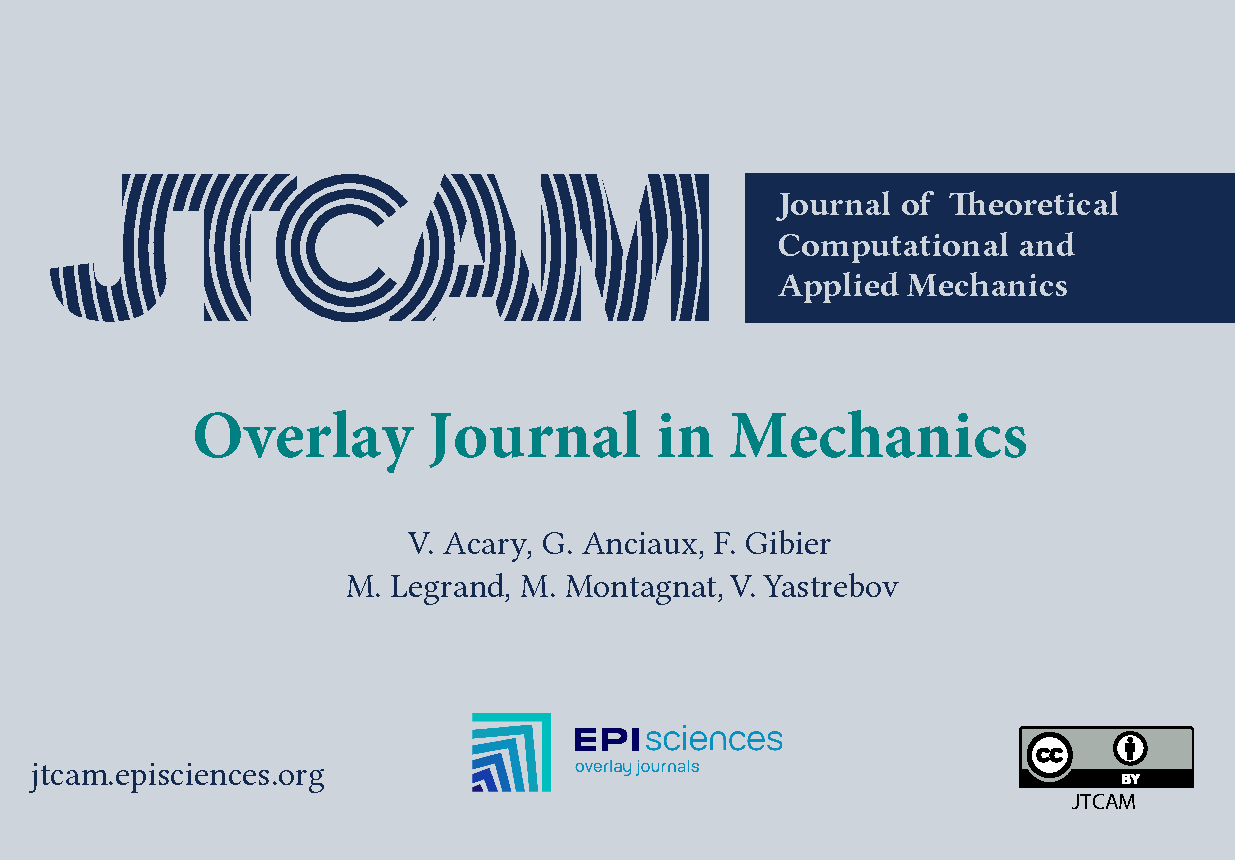
\includegraphics[width=12.8cm,height=9.6cm]{cover2.pdf}}{\begin{frame}[t,plain]\end{frame}}
% %%%%%%%%%%%%%%%%%%%%%%%%%%%%%%%%%%%%%%%%%%%%%%%%%%%%%%%%%%%%%%%%%%%%%%%%%%%%%%%%%%


\usebackgroundtemplate{\includegraphics[height=10cm]{bg.pdf}}

%%%

\begin{frame}[t]%
 \titleframe{What is an Overlay Journal?}\vskip1cm%
 \begin{center}%
 \only<1>{\fig{1}{epirevue_0c}}%
 \only<2>{\fig{1}{epirevue_1c}}%
 \only<3>{\fig{1}{epirevue_2c}}%
 \only<4>{\fig{1}{epirevue_3c}}%
 \only<5>{\fig{1}{epirevue_4c}}%
 \only<6>{\fig{1}{epirevue_5c}}%
 \end{center}%
\end{frame}
 
%%%

\begin{frame}[t]
 \titleframe{Motivation \& Chronology}\vskip0.6cm

{\centering$\to$\;\textbf{To offer an ethical and open publication model}}\\[1em]

%\textbf{Historique}
 \begin{itemize}
  \item \parbox{1.5cm}{2015/09} First discussion between VA \& ML\\[.5em]
  \item \parbox{1.5cm}{2017/07} Online discussion with interested contributors\\[.5em]
  \item \parbox{1.5cm}{2018/05} Steering committee (title, logo, etc)\\[.5em]
  \item \parbox{1.5cm}{2019/06} Scientific committee (25 members)\\[.5em]
  \item \parbox{1.5cm}{2020/01} JTCAM accepted by the Episciences plateform\\[.5em]
  \item \parbox{1.5cm}{2020/05} Editorial committee (10 members)\\[.5em]
  \item \parbox{1.5cm}{2020/08} Official JTCAM kick-off\\[.5em]
  \item \parbox{1.5cm}{2020/09} First submission
  \item \parbox{1.5cm}{2022/10} Referenced in DOAJ
 \end{itemize}

\end{frame}

%%%

\begin{frame}[t]
\titleframe{Research Community}\vskip0.6cm
\begin{itemize}
 \item Solid Mechanics
 \item Not well aware of Open Access good practices
 \item Wide spectrum: theoretical, applied, numerical, experimental
 \item Classical journals and publishers
 \begin{itemize}
 \item IJP, JMPS, IJSS, CMAME, IJMM, TI, IJES, Wear, ActaMat (Elsevier)
 \item IJNME, Adv Mat (Wiley)
 \item Comp Mech, Meccanica (Springer)
 \item PRS (Cambridge)
 \item Mechanics of Adv Mat and Struct (Taylor \& Francis)
 \end{itemize}
 \item Alternate journals (Diamond Open Access)
  \begin{itemize}
 \item CRAS (Mersenne)
 \item Archives of Mechanics (since 1950)
 \item Technische Mechanik
 \item Mathematics and Mechanics of Complex Systems (half-diamond)
 \item JACM
 \item ACM
 \end{itemize}
\end{itemize}

\end{frame}

%%%

\begin{frame}[t]
 \titleframe{JTCAM specific features}\vskip0.6cm
 \begin{itemize}
  \item \textbf{Overlay Journal}
  \begin{itemize}
  \item Always a preprint shared on Open Archives (even for refused papers)
  \item Diamond Open Access
  \end{itemize}
  \item \textbf{Team}
  \begin{itemize}
  \item Technical board: creators of the journal + data/software editor
  \item Scientific Board: invited
  \item Editorial board: elected
  \item Collegial decisions, no editor in chief
  \end{itemize}
	\item\textbf{Open Review}
	\begin{itemize}
    \item Valued Open Reviews and reviewers' work
	\end{itemize}
  \item \textbf{Copy-editing}
  \begin{itemize}
  \item Very high quality
  \item Links to open data sets and software $\to$ Reproducible research!
  \item Script to check the correctness of bibliographic entries
  \end{itemize}
 \end{itemize}

\end{frame}

%%%

% \begin{frame}[t]
 % \titleframe{Copy-editing}

 % \begin{center}
 % % FIGURES
  % \only<1-2>{\textbf{Figures de qualité TikZ}\\[2em]
    % \only<1>{Example de figure soumise en bitmap\\\fig{1}{Fig_geometry_a.png}\\}
    % \only<2>{Figure refaite vectorielle\\\fig{1}{Fig_geometry_b}\\}
  % }
 % % Tables
  % \only<3>{\textbf{Tableaux de qualité}\\[1em]
	% \fig{0.8}{table_1}
  % }
 % % References
  % \only<4->{\textbf{Références vérifiées et complétées}\\[1em]
	% \only<4>{\fig{0.8}{references}\\}
	% \only<5>{\fig{0.8}{references2}\\}
  % }
% \end{center}  

% \only<5>{
% \begin{itemize}
% \item $ $\parbox{1.5cm}{[DOI]} - DOI classique
% \item $ $\parbox{1.5cm}{[OA]} - si l'article est accessible en AO
% \item $ $\parbox{1.5cm}{[ARXIV]} - lien arXiv
% \item $ $\parbox{1.5cm}{[HAL]} - lien HAL
% \end{itemize}}
 
% \end{frame}

%%%

% \begin{frame}[t]
 % \titleframe{Bilan}\vspace{1em}
 
 % \begin{itemize}
  % \item First submission in September 2020
  % \item Fall 2022 référencé dans DOAJ
  % \item Aujourd'hui:
 % \begin{itemize}
  % \item \parbox{0.5cm}{\textbf{48}} soumissions 
  % \item \parbox{0.5cm}{\textbf{24}} articles publiés
  % \item \parbox{0.5cm}{\textbf{\;6}} articles rejetés
  % \item \parbox{0.5cm}{\textbf{18}} articles en cours de relecture / publications\\[2em]
 % \end{itemize}
 % \item JTCAM a co-répondu (portage Episciences) à l'AAP 2023 du FNSO pour pérenniser le modèle économique de la revue en externalisant le copy-editing
 % \end{itemize}
% \end{frame}

%%%

\begin{frame}[t]
 \titleframe{Challenges}\vskip0.6cm
 \begin{itemize}
  \item 24 articles published
   \begin{itemize}
   \item 22 from France (90\%)
   \item 1 from Netherlands
   \item 1 from Germany
   \item 1 from England/USA
   \end{itemize}
  \item Lack of Open Data/Open Software culture
  \item Copy-editing
 \begin{itemize}
  \item Low motivation on authors' side
  \item Lots of work for technical editors (about 10h of work per paper)
  \item Fairly long time between acceptation and publication 
 \end{itemize}
 \end{itemize}
\end{frame}

%%%

% \begin{frame}[t]
 % \titleframe{Equipe noyau} 
 % \vspace{2em}
 % \begin{center}\large
 % {\color{blue!50!black}\texttt{jtcam.episciences.org}}
 % \\[2em]
 % \fig{0.7}{equipe2}
 % \end{center}
% \end{frame}

%}

\end{document}
